\chapter{Future Work}
\label{ch:future-work}

\section{Model Improvements}

The model proved to be flexible enough to enable easy implementation of the base classes and the declaration of different agent types and resources. The area that has been least developed is related with simulation. As explained in section \ref{sec:running-sim} there is no formalisation related to simulations. This did not prove to be of any inconvenience during the creation and execution of the simulations for this paper. 

However, for users who are less acquainted with the model and its implementation it could prove to be a challenge to write simulations and collected data from them. More important is the fact that managing all the elements that compose a simulation would be very challenging for the users less experienced to the Java language itself.

\subsection{Simulation handler}

Formalising the simulations and data acquisition by the use of interfaces is necessary. The would remove from the user the responsibility of creation and management of all elements necessary to run simulations. This could be done by the creation of a \emph{simulation handler} that would contain all the necessary data objects, such as the environment (grid of nodes), list of agents, simulation renderers and the necessary methods to schedule data collection, execution of chemical stimulus renderers and so forth.

\subsection{Ant agent navigation improvements}

When it came to implement the different agents from the different casts, the biggest challenge faced was to create an algorithm to take the agents back to their nest. The method implemented in this paper (see sections \ref{sec:ant-memory}, \ref{task:find-home-hide} and \ref{task:find-home-hide}) should be improved in order to be used in more complex and longer simulations. In some cases the simulations would have a high rate of ants not finding their nest at all.

A possible improvement is to bring chemical landmarks to the model. An agent type could be created for this. This type could have properties that would point the ants to the right direction to the nest.

\subsection{Nests As Agents}

As seen in section \ref{sec:ant-nest} nest are represented as agents. On the one hand this facilitates their declaration and use as they enjoy all the infrastructure already in place for agents. On the other hand they are punctual, that is, they are placed in a node as any other agent and the other agents can see their nests only if they reach the same node at which the nest is placed. This is clearly a disadvantage and it does not reflect the reality of natural nests also.

An improvement to the model, that could be used to solve the problem of nests being punctual, could be an new interface to declare \emph{node types}. A node would have a type in the same way agents have. This would open up opportunity to create far more complex environments that it is possible now. For instance, a node could be an  \emph{obstacle} type, agents would not be allowed in there, or even a node could be a chemical landmark. With nodes having types, nests could be modelled as a set of nodes of the \emph{nest type}. This nodes would form a rectangular shape grid, in which if an agent reach any of the nodes they would be able to recognise they have reached their nest.

\section{Implementation Issues}

There is room from improvement on the basic implementation of the model. The comments made in the source files should be consolidated and in some cases improved. However a major possible improvement on the basic implementation is to change the ways the nodes are connected to from the environment grid.  

Currently the nodes are connected in a \emph{four-way} fashion, each node has $4$ neighbours, one in each direction: \emph{north, east, south, west}. This creates a major limitation related to agent navigation. Agents are very unlikely to move in diagonals, as it consists in two movements, first the agent move forward and after it moves sideways. It has been observed that agents hardly would do that because they have very low probability of selecting nodes in a diagonal sequence, e.g. north, east, north, east, north, east. Thus agents generally could not find any food sources in more complex environments where they were not directly aligned to the nest where the ants departed from.

An implementation of a grid connected differently would improve the problem considerably. If nodes had $8$ neighbours instead of $4$, agents would be able to navigate directly in the diagonal. Figure \ref{fig:connection} illustrates how the nodes would be connected and all the possible directions the agents could travel towards.

\begin{figure}[H]
\myfloatalign
\subfloat[four-way connected grid]
{\label{fig:connection-a}
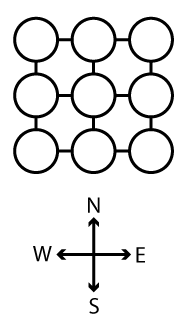
\includegraphics[width=.2\linewidth]{gfx/connection-4}} \quad
\subfloat[eight-way connected grid]
{\label{fig:connection-b}
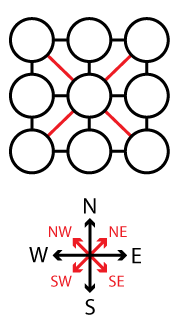
\includegraphics[width=.2\linewidth]{gfx/connection-8}}

\caption{Node connection to its neighbours}
\label{fig:connection}
\end{figure}

\section{Proposed Studies}
\label{sec:new-studies}

\subsection{Limited Number of Agents Per Node}

This experiment has the potential to explore how the formation and saturation of the pheromone trails would be affected by the limiting the number of agents that can be in a same node at the same time. From the experiment of section \ref{sec:forage-radius-inv} it is clear that in the case of a chemical communication stimulus having radius greater than $0$ agents do not follow a \emph{rational} behaviour towards their goal of foraging. As explained in the experiment discussion the node selection model is responsible for that.

It would be interesting to investigate how the trails would emerge if the nodes had a maximum number of agents allowed in that node at the same time, this would force some agents to move to nodes they would not move to otherwise, it is clear that this is the actual case in nature, as two ants cannot occupy the same physical space. 

\subsection{Improved pheromone sensing capability}

The experiment \emph{Forage Radius Investigation} (ection \ref{sec:forage-radius-inv}) has showed that the agents are too sensitive to the pheromone intensity of the direct neighbours of the node they are currently at. Again, this is due to the node selection model.

This proposed experiment would investigate how the colony forage performance and trail formation would change if agents would take in consideration not only the pheromone intensity of the neighbours of its current node but also the neighbours of the neighbours would be part of the decision process. Different 'depths' of sensibility could be experimented. This new feature would reduce the agent's sensibility to direct neighbours of its current node. 

Another possible improvement on the agent's sensing capacity would be the introduction of some sort of memory that would play part of the node selection process.